\documentclass[10pt, a4paper]{article}

\usepackage{amsmath}
\usepackage{graphicx}
\usepackage{enumitem}
\usepackage{gensymb}
\usepackage{booktabs}

\title{Eksamen - Databasesystemer våren 2025}
\author{Marius Aasgaard, Stian Hetsch}

\begin{document}

\maketitle

\section{Innledning}

Vi har hentet inspirasjon fra skisporet.no og data fra swixsport.com.

Basert på det vi finner på skisporet.no, ser vi for oss at systemet skal tillate mange destinasjoner med mange tilhørende løyper. Hver løype defineres av løypens tilhørende segmenter hva gjelder lengde, stigning og høydetap. I tillegg ønsker vi at hver løype skal inneholde informasjon om spor, altså om løypen er preparert for klassisk og/eller skøyting. Vi ser videre for oss at det med jevne mellomrom registreres løypeforhold ved hver destinasjon i form av temperatur og snøtype. Identifiserte nøkkelattributter med tanke på løypeforhold:

\begin{itemize}
	\item Destinasjon
	\item Tidspunkt for skitur 
	\item Temperatur registrert 
	\item Snøtype registrert 
	\item Løype 
	\item Spor: (klassisk, skøyting) 
	\item Segment: (lengde, stigning, høydetap)
\end{itemize}

Fra swixsport.com henter vi som sagt data, og vi ser her av de ulike skismøringene at det vil være hensiktsmessig å differensiere skismøring på navn, type, hvilke snøtyper smøringen egner seg for, temperaturintervallet definert per snøtype og hvilket brukernivå smøringen egner seg for. Nøkkelattributter som følgende:

\begin{itemize}
	\item Produktnavn på skismøring 
	\item Produktkategori: (tørrvoks, klister, glider) 
	\item Varenummer 
	\item Produktbeskrivelse
	\item Brukernivå: (nybegynner, erfaren, konkurranseløper) 
	\item Snøtype: (nyfallen, gammel, våt) 
	\item Temperaturintervall: F.eks. -10$\degree$C til -3$\degree$C 
\end{itemize}

\section{Normalisering}

Vi ser ved innhenting av data at vi ender opp med nøkkelattributter som ikke utelukkende inneholder atomære verdier. Dette gjelder både for produkt og destinasjoner (inkl. løypeforhold slik vi har valgt å løse oppgaven).

\begin{table}[h!]
\begin{tabular}{l}
Skismøring: \\
\small{(VP45, Festevoks, VP45-V), (-5 til -1, -8 til -3),} \\
\small{(Nyfallen snø, gammel snø), (Nybegynner, Erfaren, Konkurranseløper)}
\end{tabular}
\end{table}

\begin{table}[h!]
\begin{tabular}{l}
Løypeforhold: \\
\small{Sjusjøen, 21.04.2025 13:21, -4, Nyfallen snø, Elgåsen, (Klassisk, Skøyting)} \\
\small{((600, 9.5, 2.7), (200, 0, 7.7), (100, 0.7, 0.6))}
\end{tabular}
\end{table}

\subsection{1NF - Første normalform}

I følge Databasesystemer (Kristoffersen, 2021, s. 240) er en relasjonsmodell i første normalform når alle attributter inneholder atomære verdier, og ingen gjentatte grupper forekommer. Dette innebærer at hver kolonne inneholder én verdi per rad, og at man unngår lister, delte felter eller strukturerte felt i én celle.

Utgangspunktet vårt brøt med krav til 1NF ved flere anledninger: \\

Smøringstabellen hadde felt som inneholdt flere brukernivåer og flere snøtyper i samme celle. Produktet i seg selv var også en sammensatt attributt.

Løypeforhold inneholdt flere sportyper per løype som tekst, og segmentene var lister i en liste.

For å oppfylle krav til 1NF gjorde vi følgende grep:

Løypeforhold: Splittet opp tabell i hensiktsmessige kolonner, slik at det heller blir mange rader med atomære verdier.
Smøring: Gjort tilsvarende grep som i løypeforhold

Disse tiltakene fjernet alle flerverdige attributter og gjentatte grupper, i tråd med teorien om 1NF. Resultatet er en struktur med én verdi per celle og ett datasett per rad, slik relasjonsmodellen forutsetter.

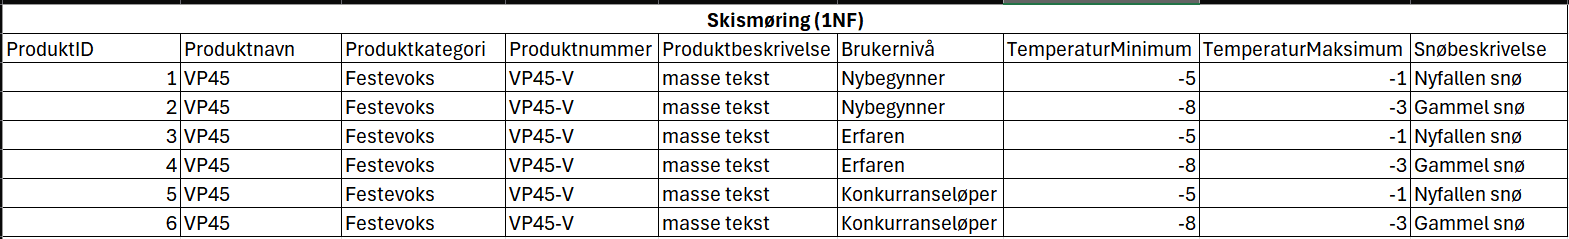
\includegraphics[width=\textwidth]{skismoring_1nf.png} \\

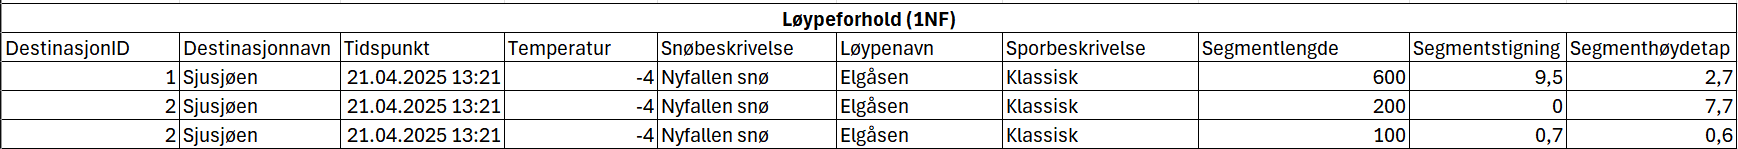
\includegraphics[width=\textwidth]{loypeforhold_1nf.png}

Vi identifiserer deretter de partielle avhengighetene

Løypeforhold:

\begin{itemize}
	\item DestinasjonID $\rightarrow$ DestinasjonNavn 
	\item DestinasjonID, LoypeID $\rightarrow$ Sporbeskrivelse 
	\item DestinasjonID, Tidspunkt $\rightarrow$ Temperatur, Snobeskrivelse
	\item LoypeID $\rightarrow$ LoypeNavn
	\item LoypeID, SegmentID $\rightarrow$ SegmentLengde, SegmentStigning, SegmentHoydetap 
	\item SportypeID $\rightarrow$ Sporbeskrivelse 
\end{itemize}

Smøring:

\begin{itemize}
	\item ProduktID $\rightarrow$ ProduktNavn, ProduktKategori, ProduktNummer, Produktbeskrivelse, Snotype, Brukerniva
	\item ProduktID, Snotype $\rightarrow$ TemperaturMinimum, TemperaturMaksimum 
	\item Snotype $\rightarrow$ Snobeskrivelse 
	\item Brukerniva $\rightarrow$ Brukernivabeskrivelse
\end{itemize}

\subsection{2NF - Andre normalform}

Som nevnt innledningsvis, forutsetter vi at løypeforhold registreres med jevne mellomrom, det vil si at det ikke er mulig å registrere to forskjellige temperaturer og/eller snøtyper på samme tidspunkt, på samme destinasjon.

Ifølge Databasesystemer (Kristoffersen, 2021, s. 241) er en relasjonsmodell i andre normalform når den allerede er i 1NF, og ingen ikke-nøkkelattributter er delvis funksjonelt avhengige av en sammensatt primærnøkkel.

I vårt tilfelle hadde både løypeforhold og smøring slike delvise avhengigheter.

Løypeforhold:

Attributter som LoypeNavn og DestinasjonNavn var kun avhengige av henholdsvis LoypeID og DestinasjonID, og ble derfor flyttet til egne tabeller.

Segmentdata ble tidligere lagret som lister, men ble flyttet til en egen segment-tabell med én rad per segment.

Sportyper ble splittet ut i en koblingstabell spor, for å fjerne flerverdige felt.

Smøring:

Temperaturintervall var delvis avhengig av snøtype. Vi flyttet snøtype til egen tabell.

Resultatet er at alle ikke-nøkkelattributter nå er fullt funksjonelt avhengige av hele primærnøkkelen i tabellene, i tråd med kravet til 2NF.

\begin{itemize}
	\item Destinasjon(\underline{DestinasjonID}, DestinasjonNavn)
	\item Loype(\underline{LoypeID}, DestinasjonID*, LoypeNavn) 
	\item Segment(\underline{SegmentID}, LoypeID*, Lengde, Stigning, Hoydetap) 
	\item Sportype(\underline{SportypeID}, Sporbeskrivelse)
	\item Spor(\underline{SporID}, LoypeID*, SportypeID*)
	\item Snotype(\underline{SnotypeID}, Snobeskrivelse) 
	\item Loypeforhold(\underline{DestinasjonsID*}, \underline{Tidspunkt}, Temperatur, SnotypeID*)
	\item Produktkategori(\underline{ProduktkategoriID}, Produktkategoribeskrivelse) 
	\item Smoring(\underline{ProduktID}, \underline{BrukernivaID*}, \underline{SnotypeID*}, ProduktNavn, Produktkategori*, Produktnummer, Produktbeskrivelse, , TemperaturMinimum, TemperaturMaksimum) 
\end{itemize}


-- 1NF

1. DestinasjonLoype:
Primærnøkler (PK): Kombinasjon av DestinasjonID og LoypeID (komposittnøkkel siden hver kombinasjon unikt identifiserer en rad).
Fremmednøkkel (FK): DestinasjonID (peker til Destinasjon.DestinasjonID i opprinnelig modell).

2. LoypeSegment:
Primærnøkkel (PK): SegmentID (hver rad representerer et unikt segment).
Fremmednøkler (FK):
- LoypeID (peker til Loype.LoypeID).
- DestinasjonID (peker til Destinasjon.DestinasjonID).

3. LoypeSpor:

- Primærnøkkel (PK): SporID (hvert spor er unikt identifisert).
- Fremmednøkler (FK):- LoypeID (peker til Loype.LoypeID).
- DestinasjonID (peker til Destinasjon.DestinasjonID).

4. Loypeforhold
Primærnøkkel (PK): Kombinasjon av DestinasjonsID og Tidspunkt (komposittnøkkel)
Fremmednøkkel (FK): DestinasjonsID (peker til Destinasjon.DestinasjonID).

5. Smoring
Primærnøkkel (PK): SmoringID (hver smøring er unikt identifisert)
Fremmednøkkel (FK): Snotype kan potensielt kobles til LoypeforholdDenormalisert.Snotype


\begin{itemize}
	\item DestinasjonLoype(\underline{DestinasjonID}*, \underline{LoypeID}, DestinasjonNavn, LoypeNavn) 
	\item LoypeSegment(\underline{SegmentID}, LoypeID*, DestinasjonID*, LoypeNavn, SegmentLengde, SegmentStigning, SegmentHoydetap) 
	\item LoypeSpor(\underline{SporID}, LoypeID*, DestinasjonID*, LoypeNavn, Sportype)
	\item Loypeforhold(\underline{DestinasjonsID*}, \underline{Tidspunkt}, Temperatur, Snotype, DestinasjonsNavn) 
	\item Smoring(\underline{SmoringID}, Brukerniva, Snotype*, ProduktNavn, Produktkategori, Produktnummer, Produktbeskrivelse, TemperaturMinimum, TemperaturMaksimum)
\end{itemize}

-- 2NF

\begin{itemize}
	\item Destinasjon(\underline{DestinasjonID}, Navn) 
	\item Loype(\underline{LoypeID}, DestinasjonID*, Navn) 
	\item Segment(\underline{SegmentID}, LoypeID*, Lengde, Stigning, Hoydetap) 
	\item Spor(\underline{SporID}, LoypeID*, Sportype)
	\item Loypeforhold(\underline{DestinasjonsID*}, \underline{Tidspunkt}, Temperatur, Snotype) 
	\item Smoring(\underline{SmoringID}, Brukerniva, Snotype, ProduktNavn, Produktkategori, Produktnummer, Produktbeskrivelse, TemperaturMinimum, TemperaturMaksimum)
\end{itemize}

\subsection{3NF - Tredje normalform}

\begin{itemize}
	\item Destinasjon(\underline{DestinasjonID}, Navn) 
	\item Brukerniva(\underline{BrukernivaID}, Brukerniva)
	\item Loype(\underline{LoypeID}, DestinasjonID*, Navn) 
	\item Segment(\underline{SegmentID}, LoypeID*, Lengde, Stigning, Hoydetap) 
	\item Sportype(\underline{SportypeID}, Sporbeskrivelse)
	\item Spor(\underline{SporID}, LoypeID*, SportypeID*)
	\item Snotype(\underline{SnotypeID}, Snobeskrivelse) 
	\item Loypeforhold(\underline{DestinasjonsID*}, \underline{Tidspunkt}, Temperatur, SnotypeID*) 
	\item Produktkategori(\underline{ProduktkategoriID}, Produktkategoribeskrivelse) 
	\item Smoring(\underline{SmoringID}, BrukernivaID*, SnotypeID*, ProduktNavn, Produktkategori*, Produktnummer, Produktbeskrivelse)
	\item Produktegenskaper(\underline{EgenskaperID}, ProduktID*, BrukernivaID*, SnotypeID*, TemperaturMinimum, TemperaturMaksimum)
\end{itemize}




























\subsection{BCNF}

\hfill \break

\section{ER-modellering}

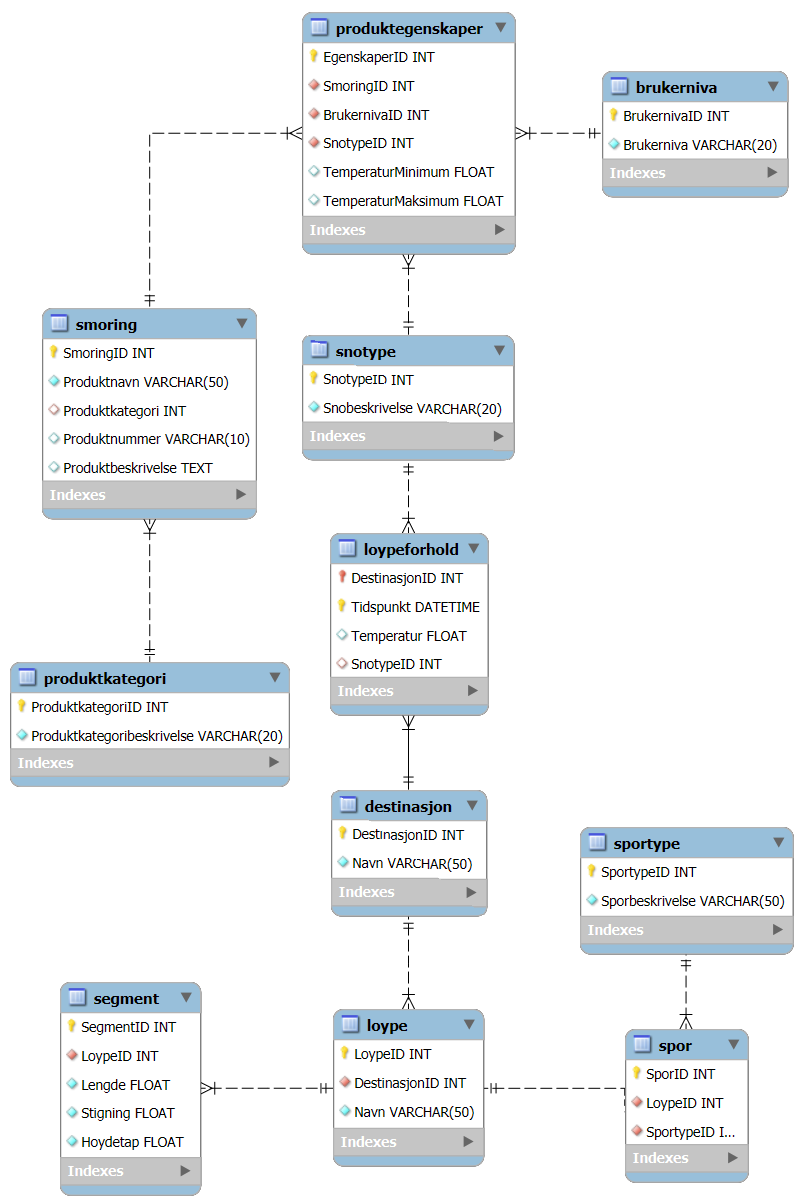
\includegraphics[width=\textwidth]{ermodell.png}

\section{Database implementasjon}

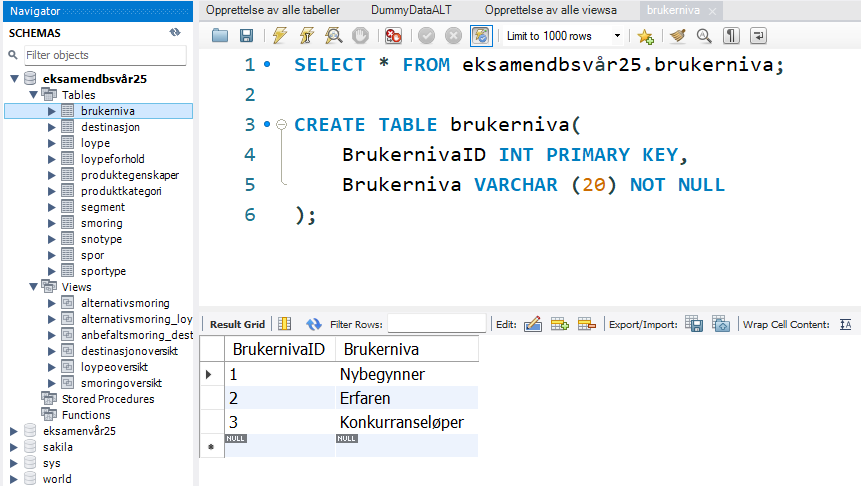
\includegraphics[width=\textwidth]{brukerniva.png}
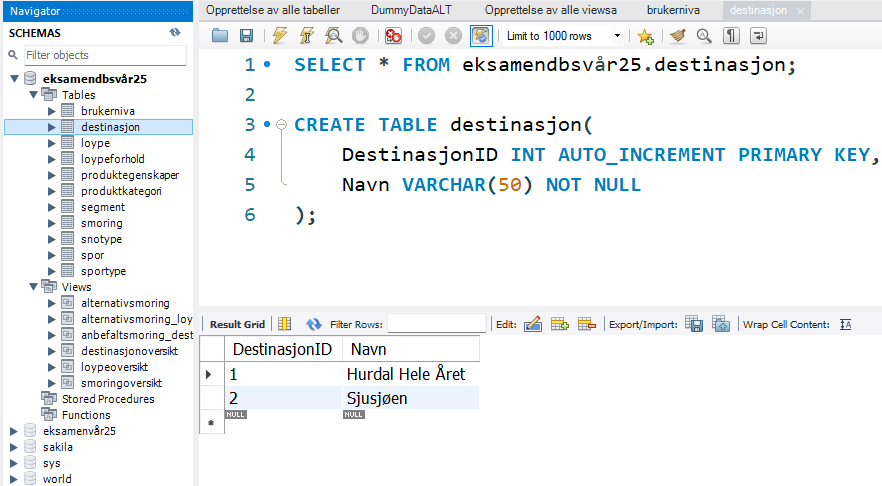
\includegraphics[width=\textwidth]{destinasjon.png}
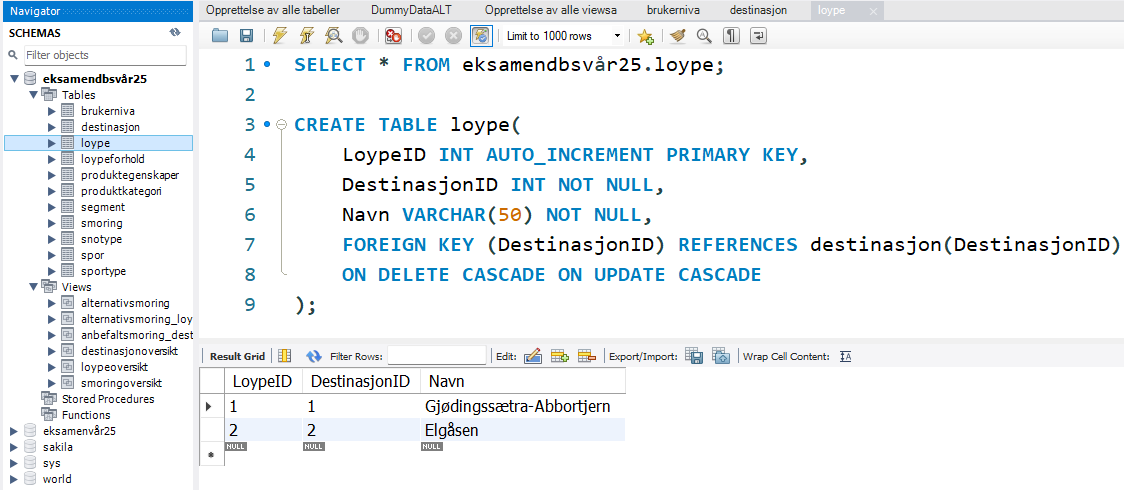
\includegraphics[width=\textwidth]{loype.png}
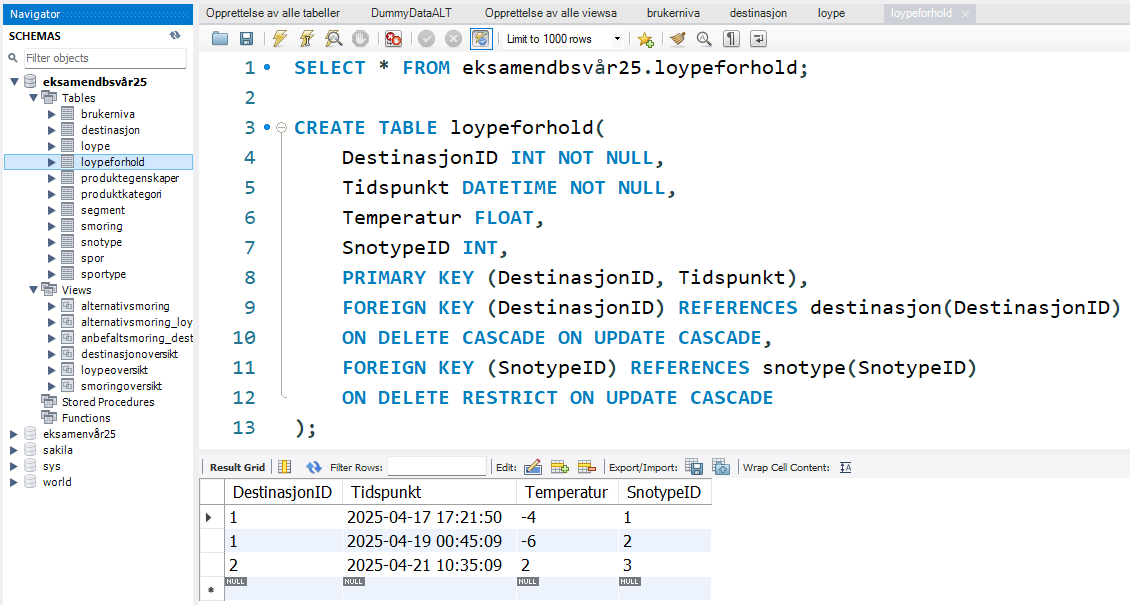
\includegraphics[width=\textwidth]{loypeforhold.png}
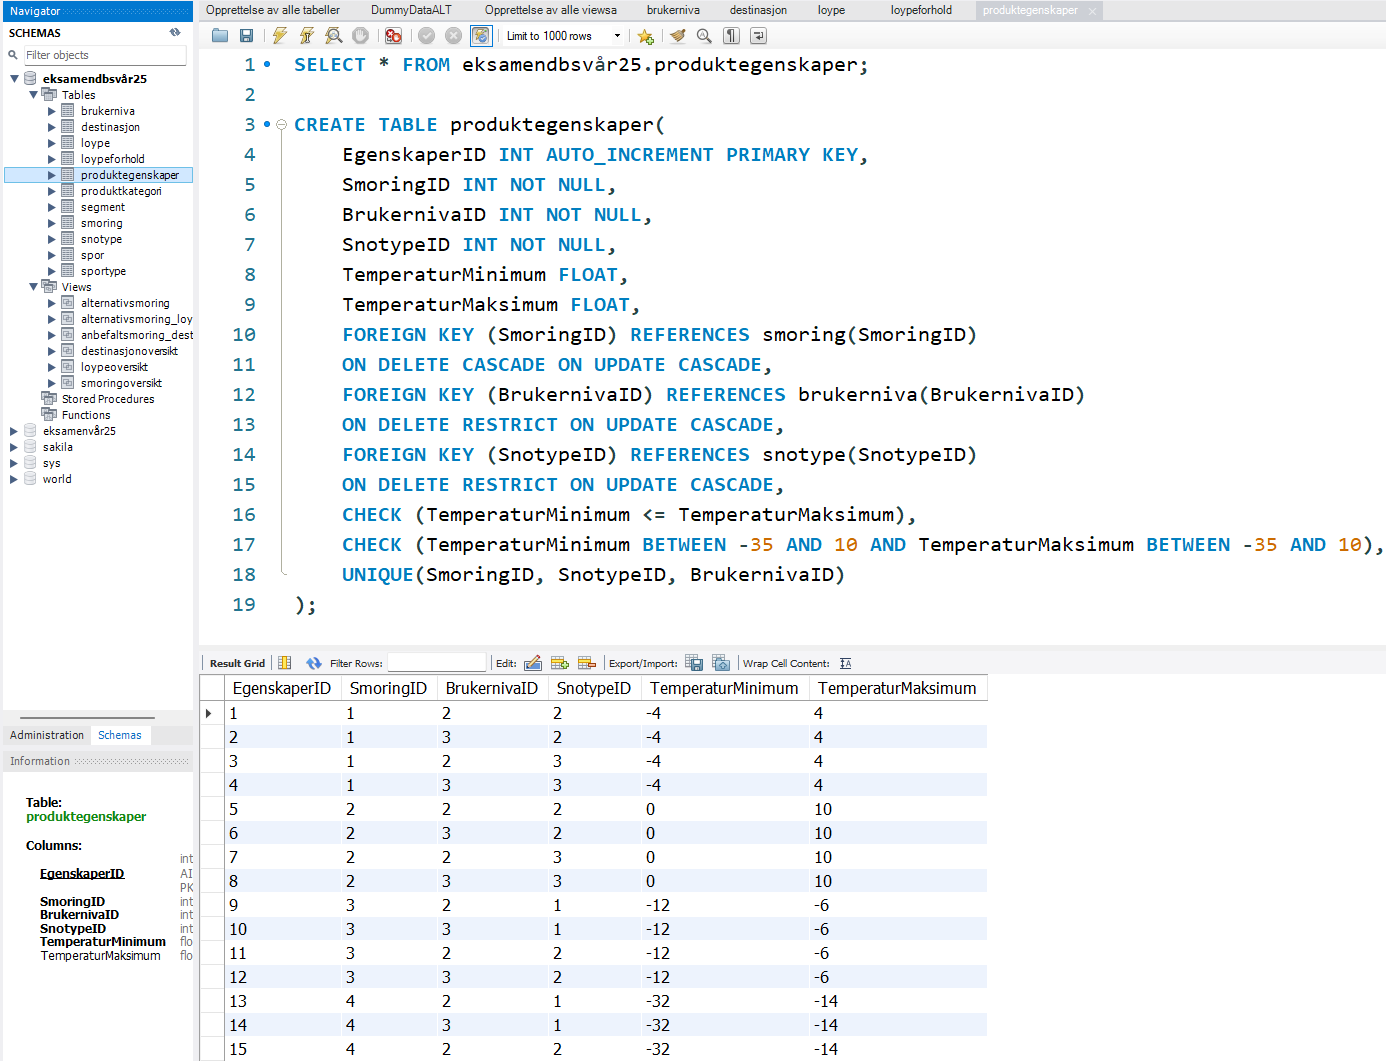
\includegraphics[width=\textwidth]{produktegenskaper.png}
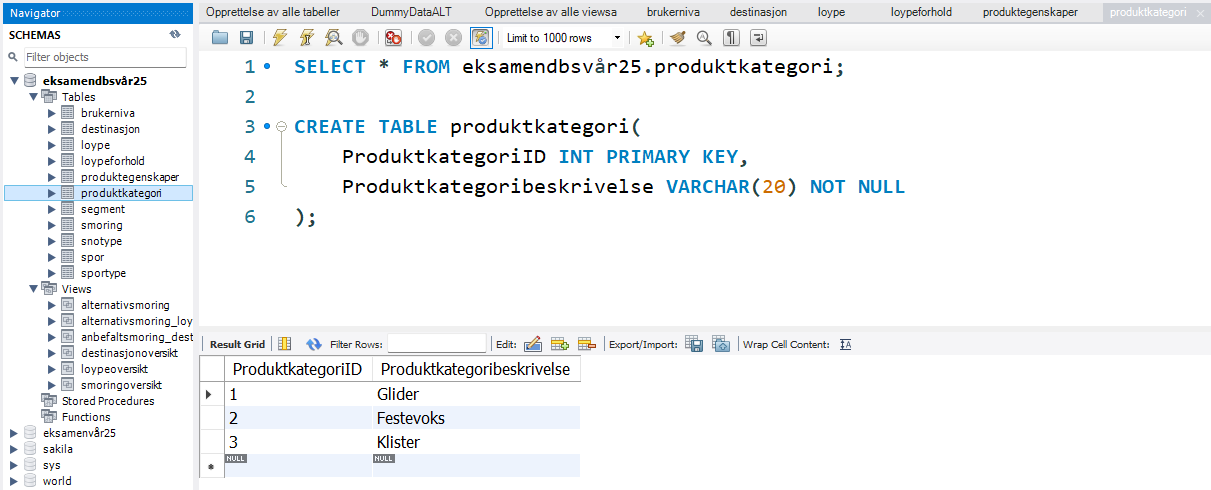
\includegraphics[width=\textwidth]{produktkategori.png}
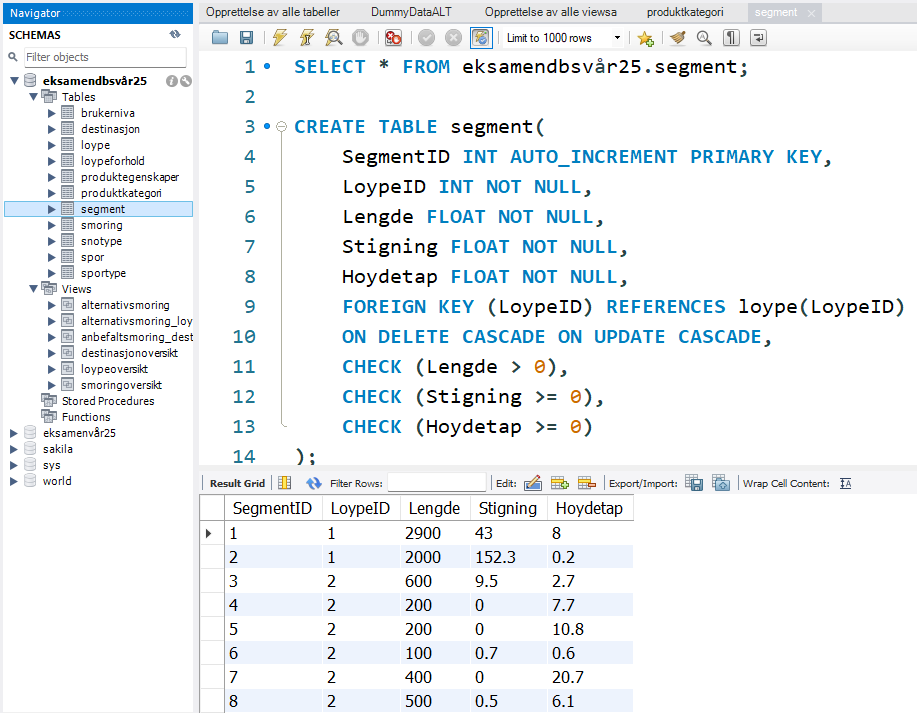
\includegraphics[width=\textwidth]{segment.png}
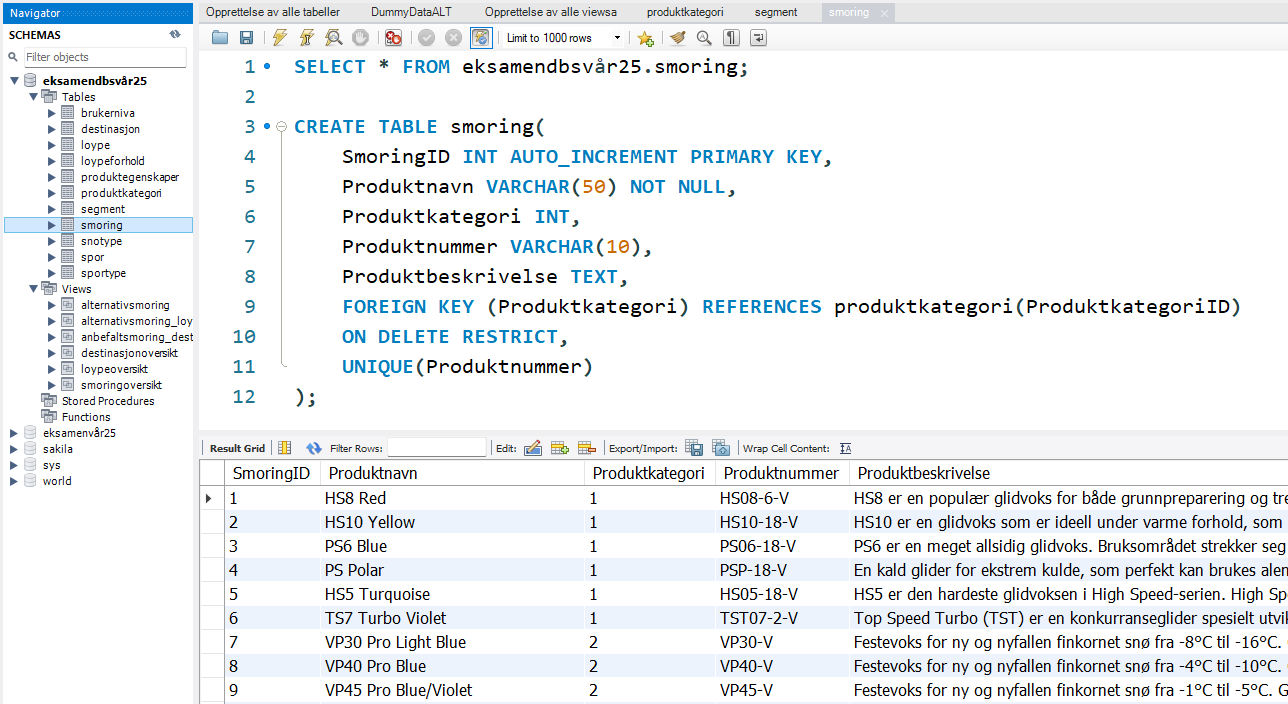
\includegraphics[width=\textwidth]{smoring.png}
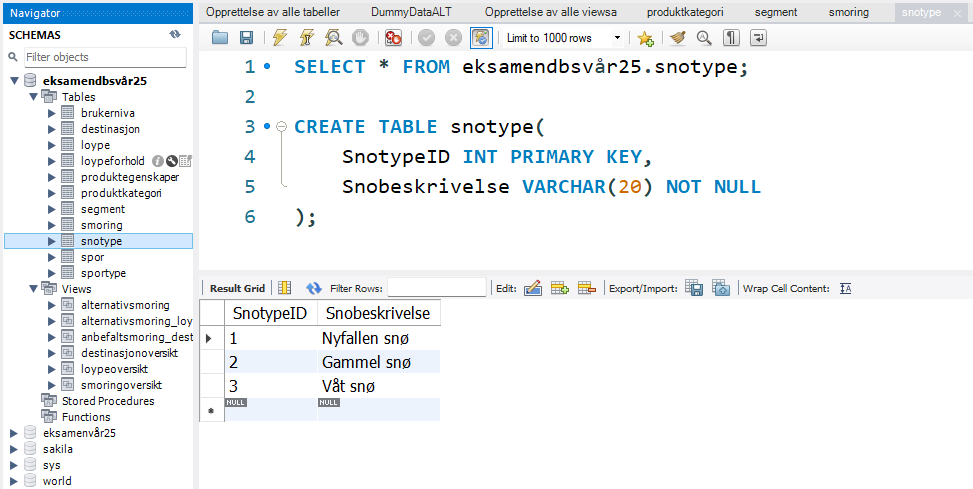
\includegraphics[width=\textwidth]{snotype.png}
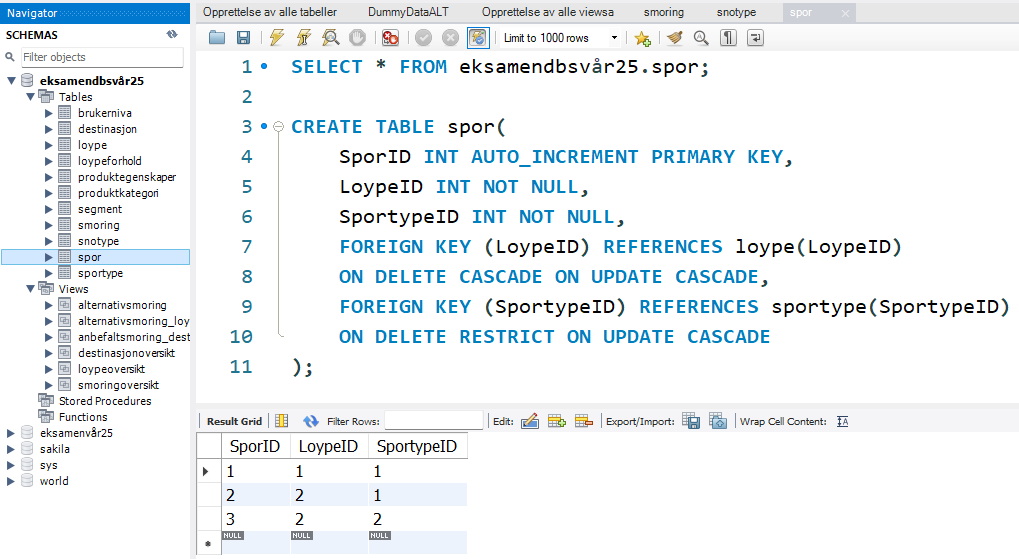
\includegraphics[width=\textwidth]{spor.png}
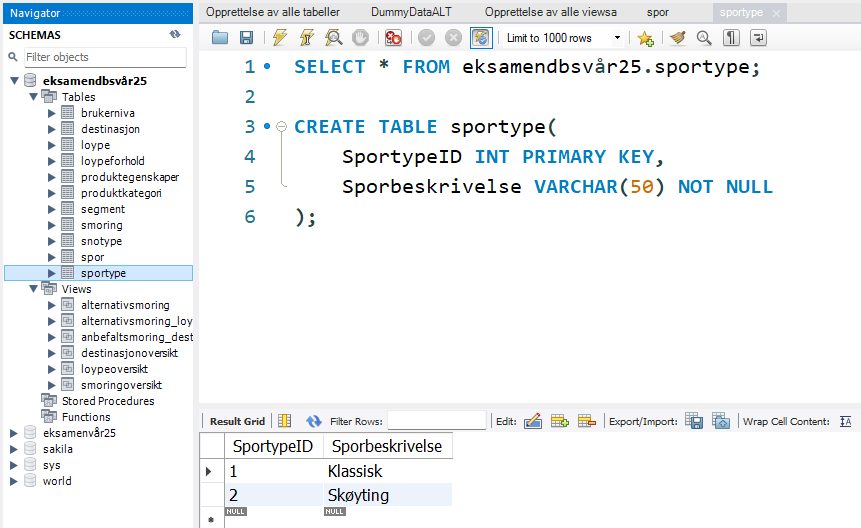
\includegraphics[width=\textwidth]{sportype.png}

\section{Dummy data}

\subsection{Begrunnelse for valg av dummydata}

Dummydataene vi har med i databasen vår er valgt basert på evnen til å demonstrere systemets funksjonalitet i tråd med kravspesifikasjonene. Dermed har vi fylt databasen med data som etter vår mening dekker hele bredden av brukerinteraksjoner i systemet - alt fra registrering av løypeforhold til valg av skismøring basert på temperatur, snøtype og brukernivå. \\

Videre har vårt valg av data som hensikt å gi oss realistiske og relevante resultater gjennom alle SQL-spørringer og views. På denne måten kan man verifisere og teste databasen sin logikk. \\

Innhold i tabellene:
\begin{itemize}
	\item Smoring inneholder 18 unike smøringer hentet fra Swix sine produkter
	\item Brukerniva inneholder tre ferdighetsnivåer som definert i oppgave
	\item Destinasjon inneholder to steder / destinasjoner, og er hentet fra skisporet.no
	\item Loype inneholder løypeinformasjon for utvalgte løyper med kobling mot destinasjon 
	\item Produktegenskaper holder på- og kobler sammen hvert produkt og de respektive egenskapene 
	\item Produktkategori inneholder de tre kategoriene som definert i kravspesifikasjon (klister, tørrvoks og glider)
	\item Segment inneholder informasjon (lengde, stigning og høydetap) om hvert segment og kobler hvert segment mot riktig løype 
	\item Snotype inneholder de tre snøtypene som gitt av kravspesifikasjon (nyfallen, gammel og våt) 
	\item Sportype inneholder klassisk og skøyting 
	\item Spor kobler sportyper til løype (som oppgitt på skisporet.no)
\end{itemize}

Vi mener med denne dataen at temperaturintervallene og snøtypene vi har med dekker de mest vanlige løypeforholdene i Norge. Det finnes smøringer og snøtyper i vår data som overlapper slik at man kan få flere anbefalninger i samme resultat. Alle kombinasjoner mellom snøtype, brukernivåer og temperaturer er representert på en måte som lar systemet gi tilpassede smøreforslag basert på disse attributtene via views og SQL-spørringer.

\section{SQL-spørringer}

\subsection{View: Smoringoversikt:}

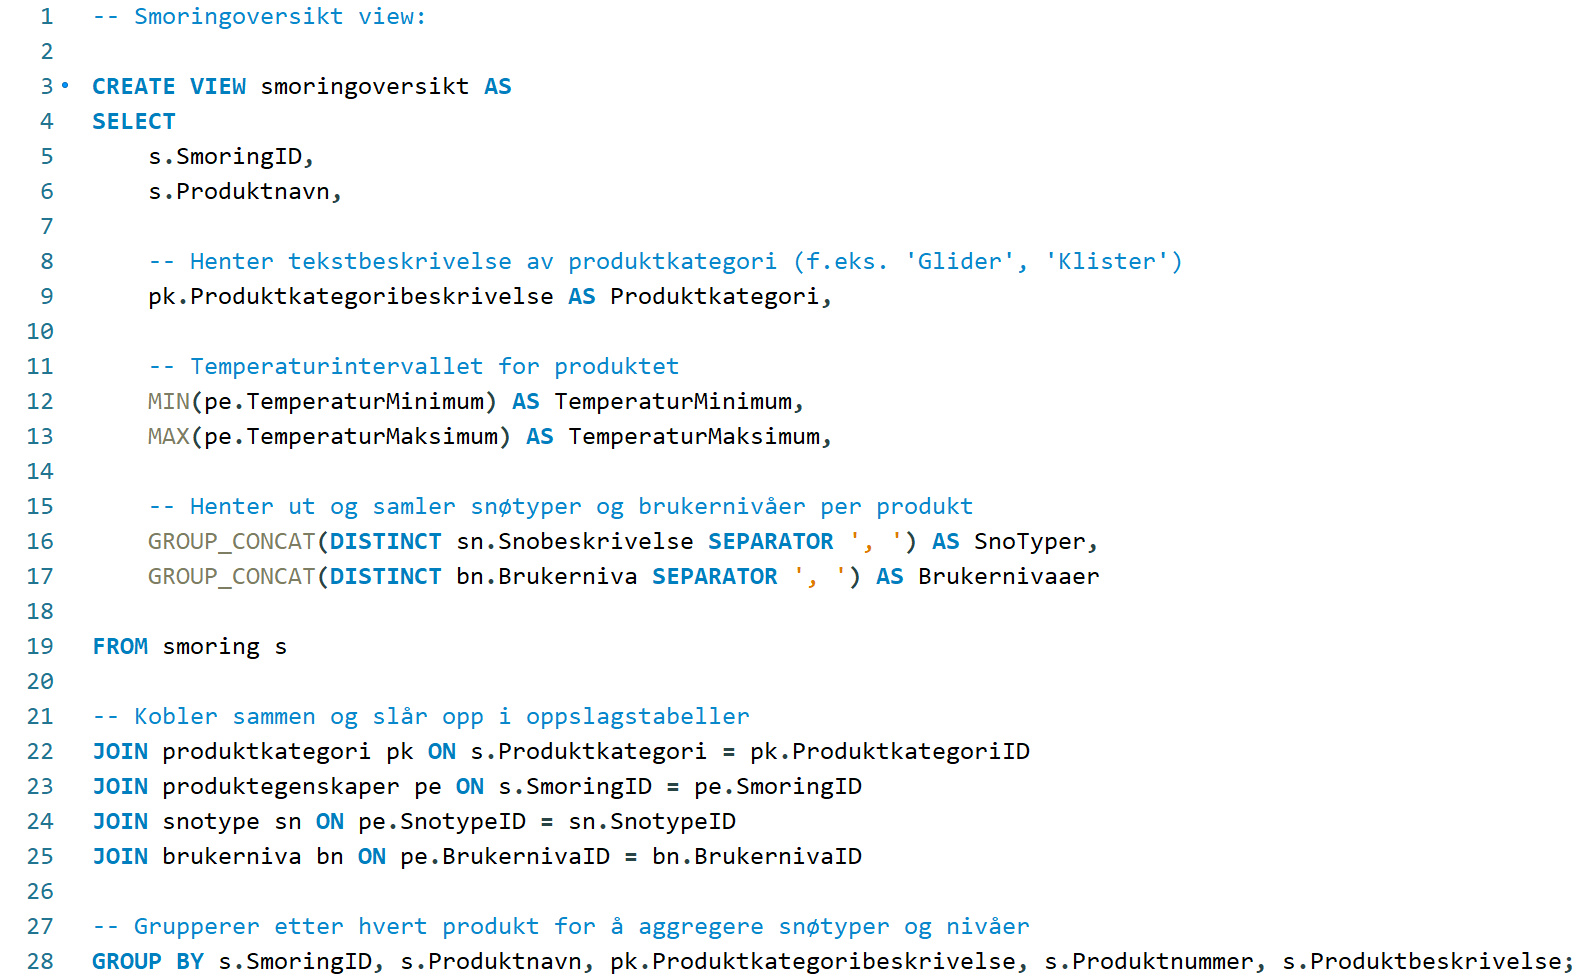
\includegraphics[width=\textwidth]{smoringoversikt.png}

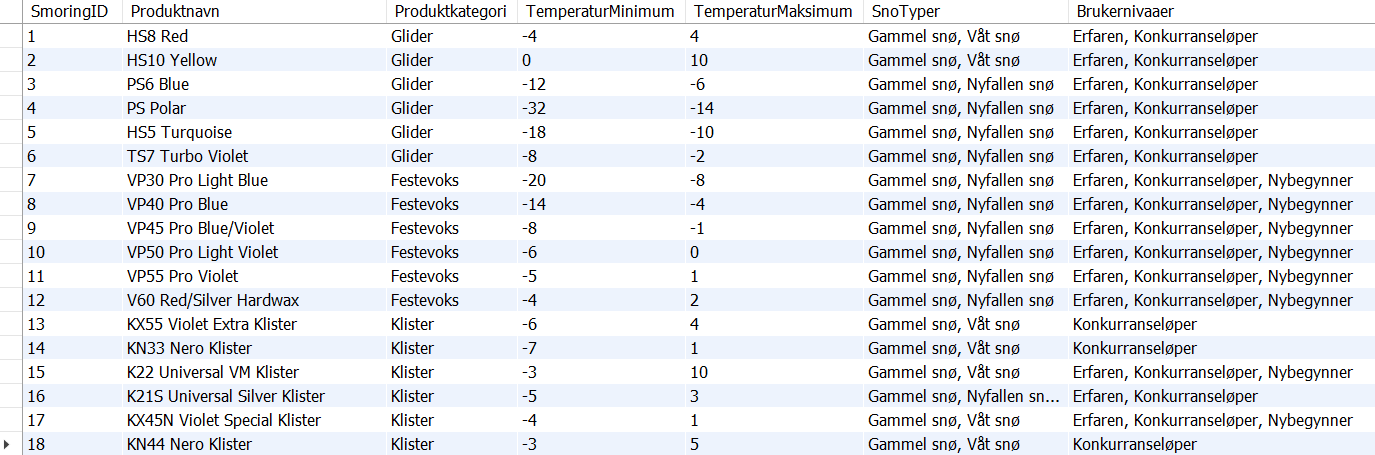
\includegraphics[width=\textwidth]{smoringoversikt_resultat.png}

Dette viewet sin hensikt er å aggregere informasjon fra flere tabeller. Det gjelder smoring, produktegenskaper, snotype og brukerniva. Viewet samler og viser all informasjon om hver smøring på én rad: navn, kategori, snøtyper, brukernivåer og temperaturintervall. Kort sagt kobler den smøringer opp mot relevante løypeforhold og brukernivåer. Dette gjør det enkelt å bruke gjeldende view videre i andre spørringer og views som skal vise anbefalninger og alternativer.

\subsection{View: Destinasjonsoversikt:}

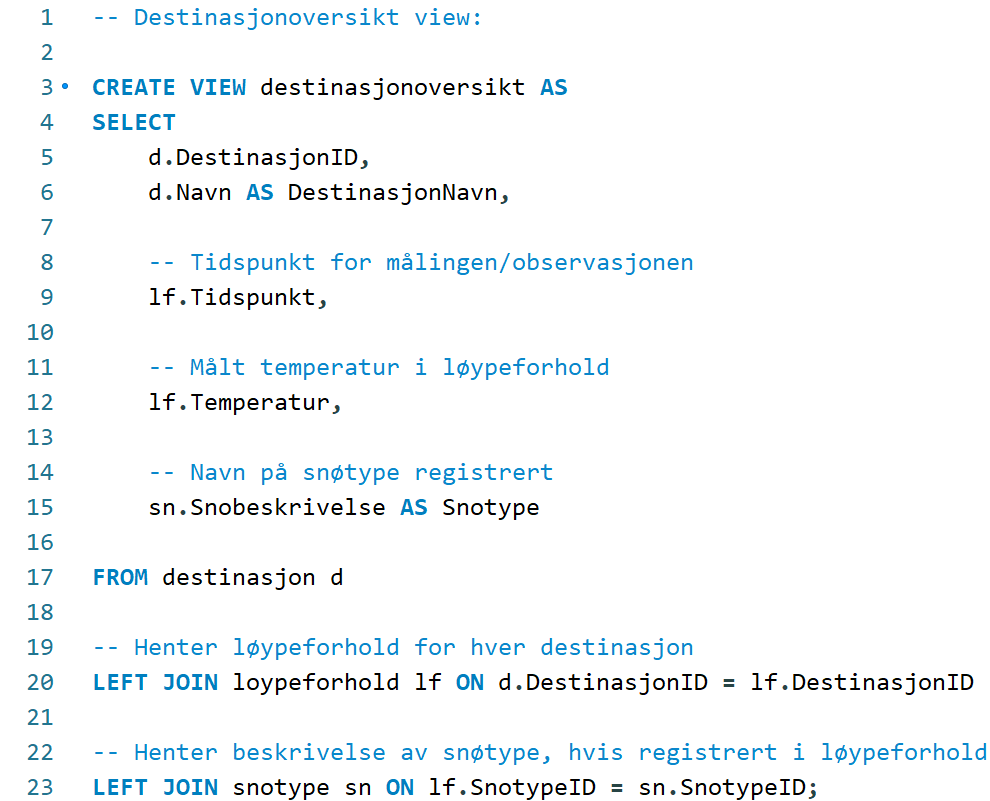
\includegraphics[width=\textwidth]{destinasjonoversikt.png}

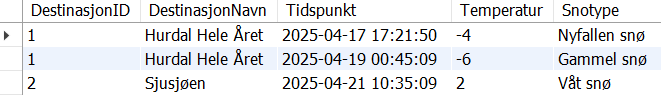
\includegraphics[width=\textwidth]{destinasjonoversikt_resultat.png}

Dette viewet sin hensikt er en forenklet oversikt som samler relevant løypeforhold for videre bruk i anbefalningssystemet. Viewet henter data fra loypeforhold, destinasjon og snotype. Videre viser det alle registrerte værforhold per destinasjon, inkludert tidspunkt, temperatur og snøtype. 

\subsection{View: Loypeoversikt:}

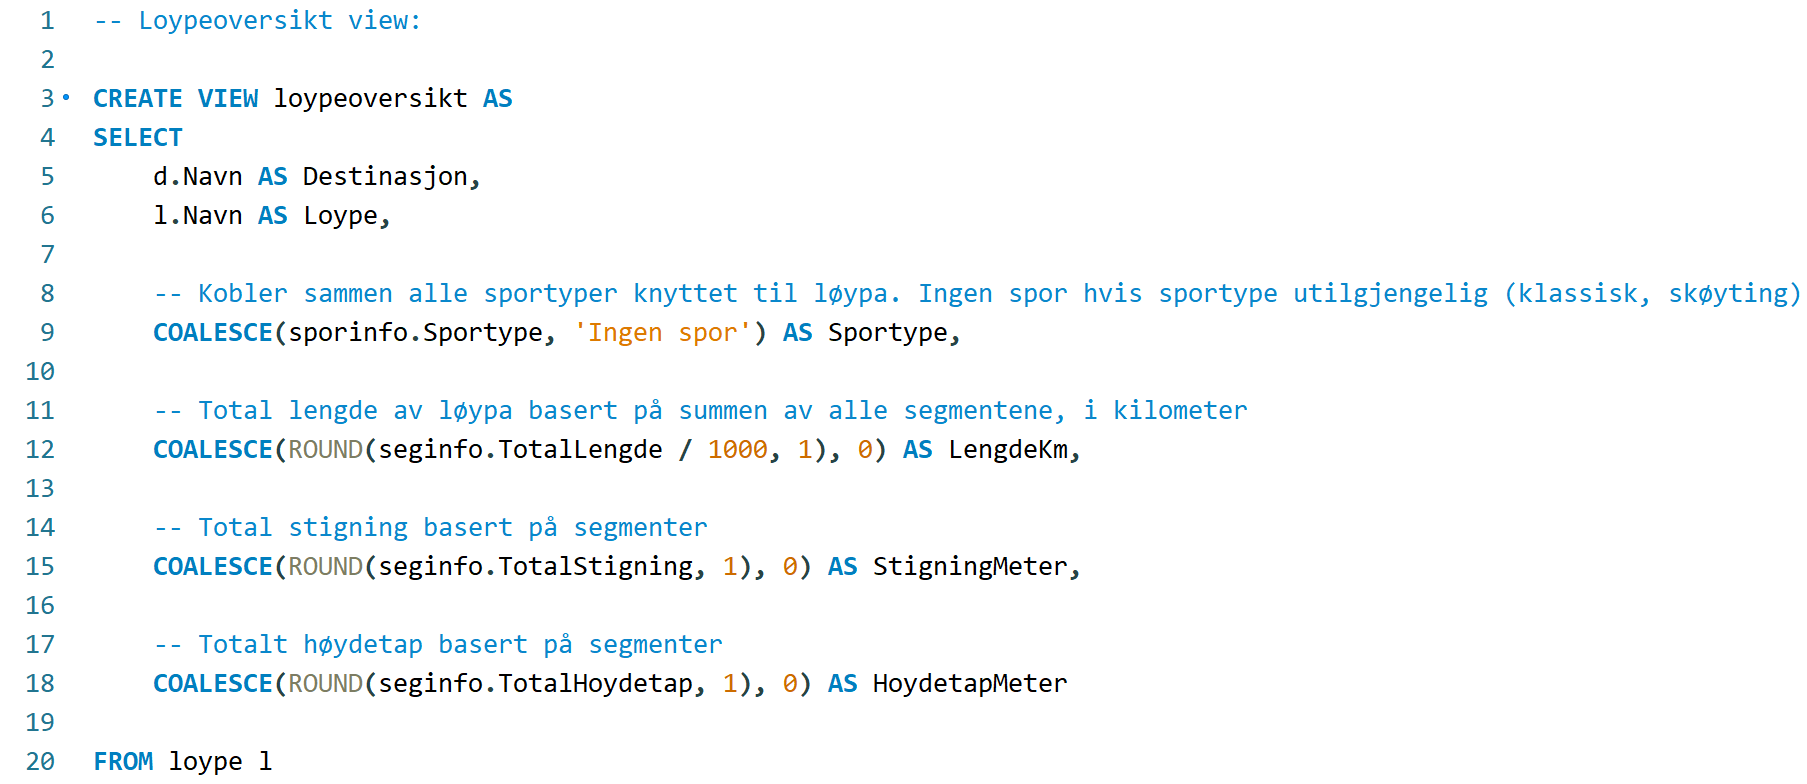
\includegraphics[width=\textwidth]{loypeoversikt_1.png}
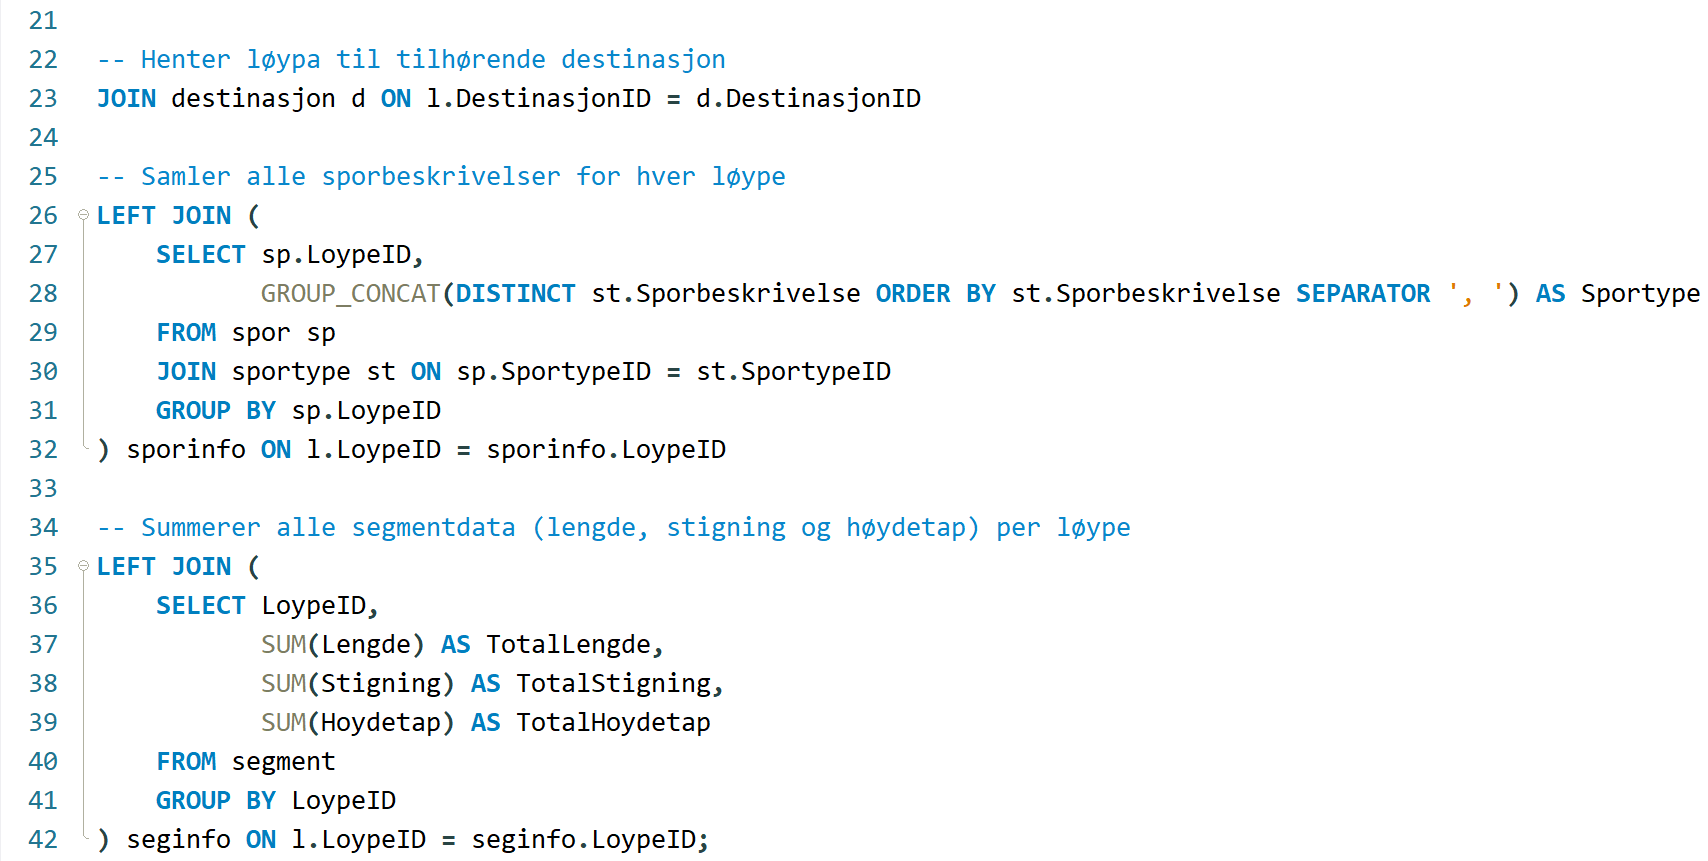
\includegraphics[width=\textwidth]{loypeoversikt_2.png}

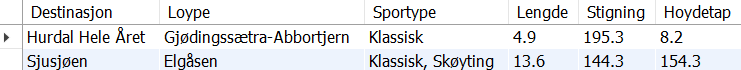
\includegraphics[width=\textwidth]{loypeoversikt_resultat.png}

	Dette viewet sin hensikt er å gi en oversikt over alle løyper i systemet, med total lengde, stigning og høydetap basert på tilhørende segmenter, samt hvilke sportyper som finnes i hver løype. For å gjøre denne informasjonen oversiktlig, summeres alle segmentdata per løype og sportyper aggregeres i en kommaseparert liste. Det gjør at hver rad i oversikten viser en god oversikt over hver løype. 

\subsection{View: Alternativsmoring:}

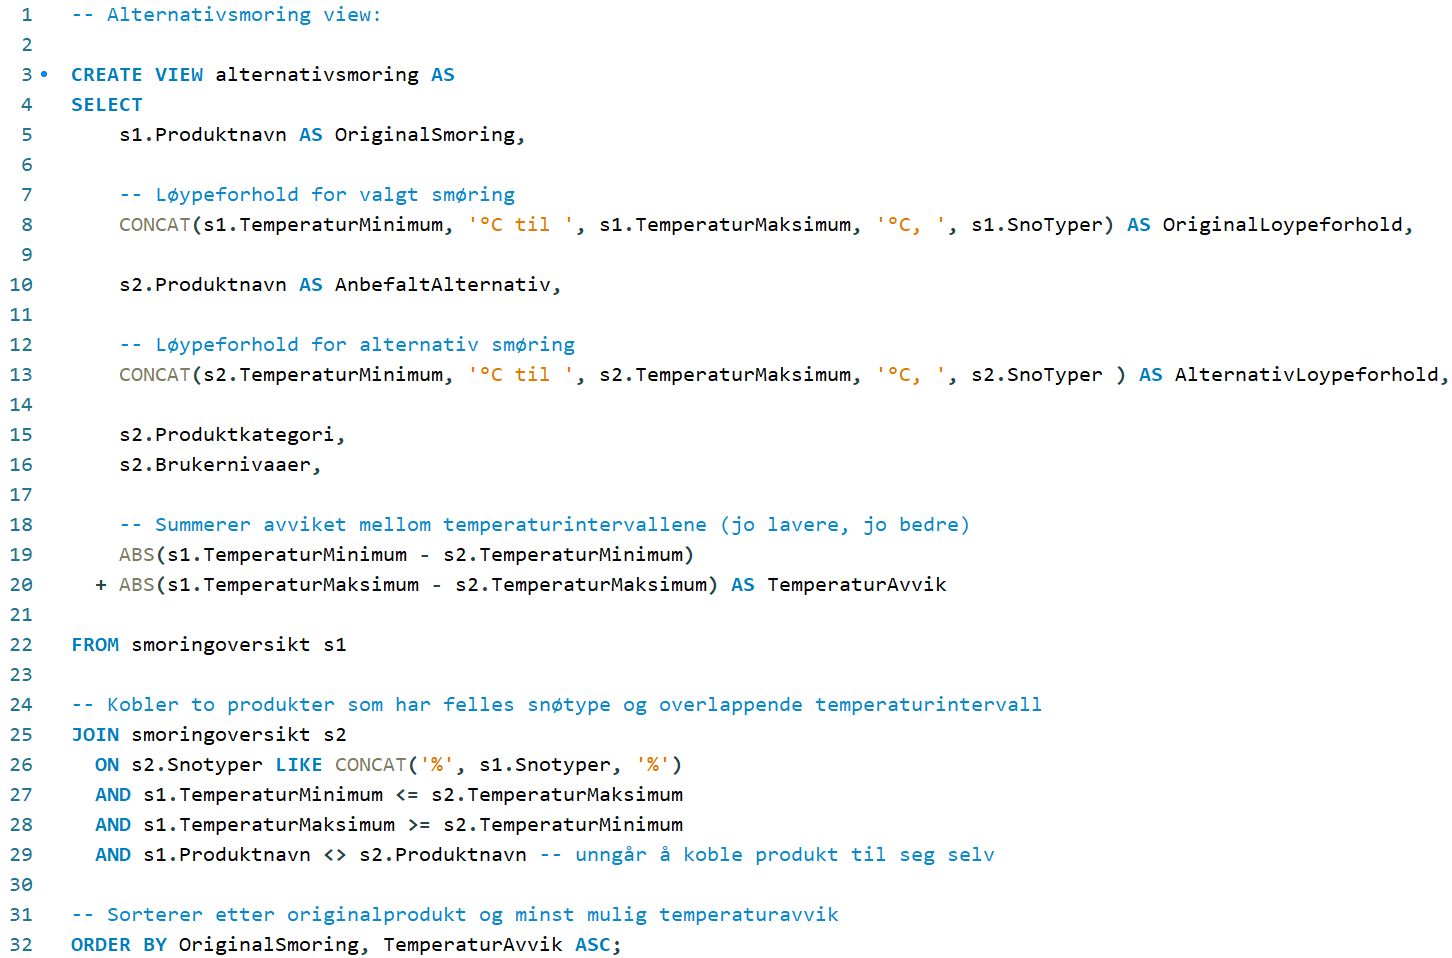
\includegraphics[width=\textwidth]{alternativsmoring.png}
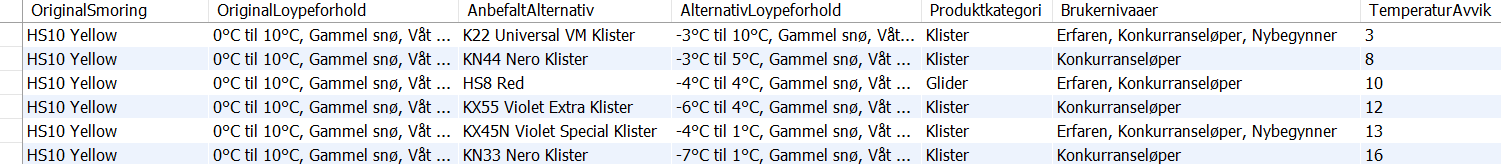
\includegraphics[width=\textwidth]{alternativsmoring_resultat.png}

Dette viewet sin hensikt er å gi en oversikt over alternative smøringer til en gitt smøring. Viewet matcher produkter mot hverandre basert på overlappende temperaturintervall og samme kategori. Resultatet sorteres etter hvor stort temperaturavviket er og inneholder både navnet på originalsmøringen, beskrivelse av forholdet og alternativene. 

\subsection{View: Alternativesmoring loypeforhold:}

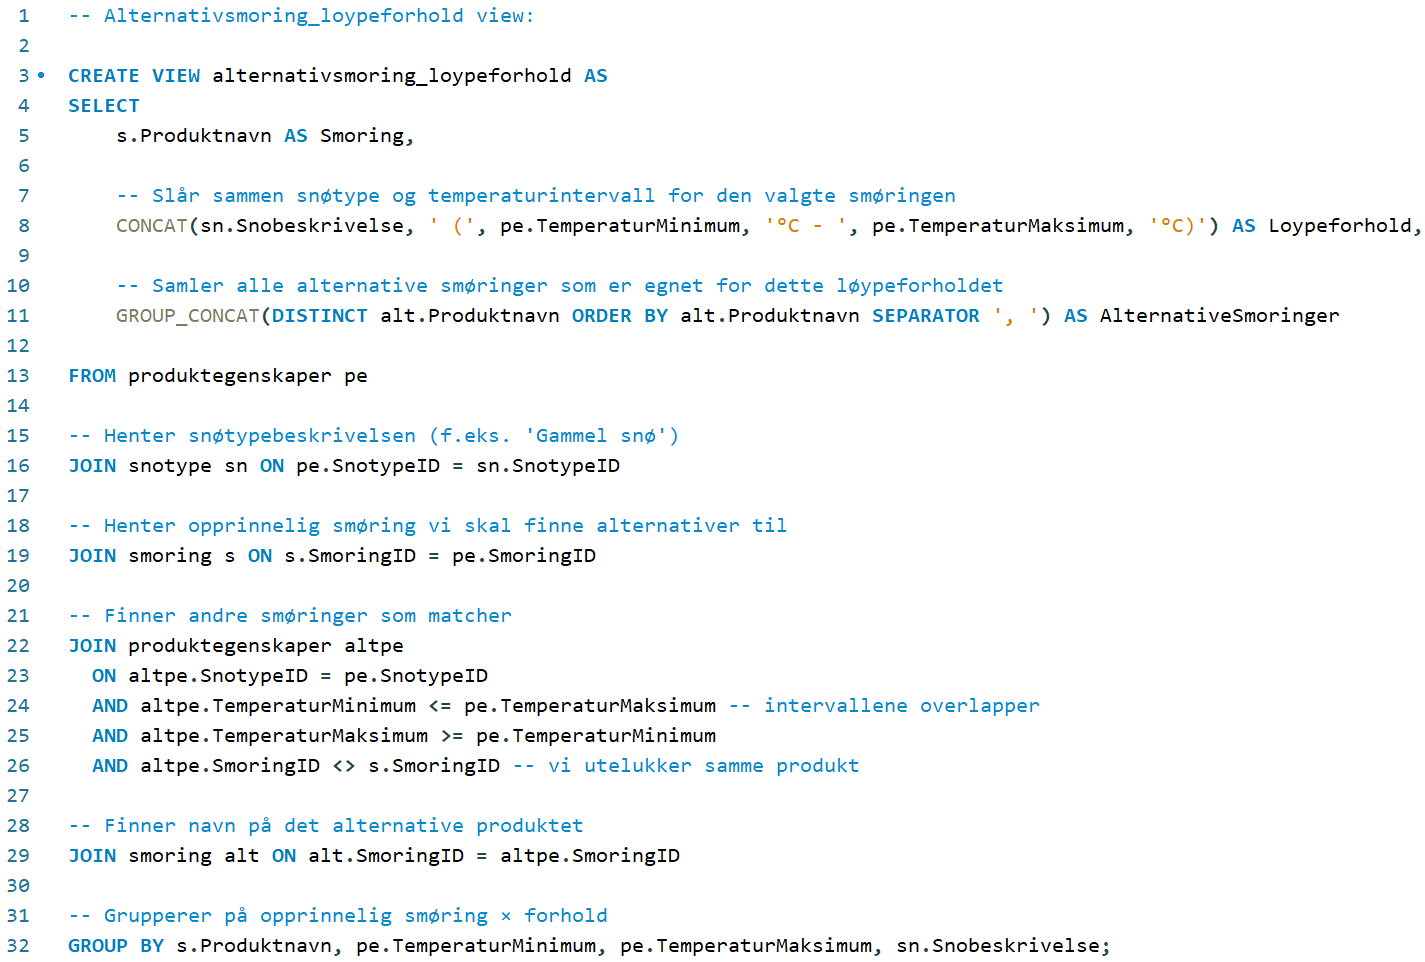
\includegraphics[width=\textwidth]{alternativsmoring_loypeforhold.png}
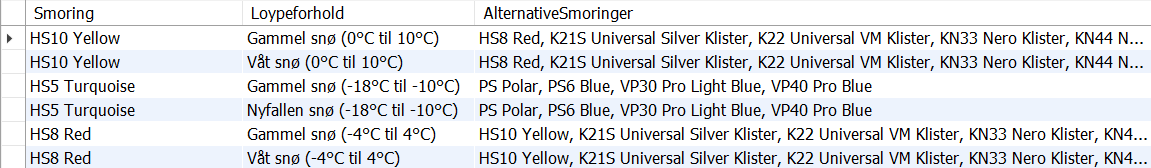
\includegraphics[width=\textwidth]{alternativsmoring_loypeforhold_resultat.png}

Dette viewet sin hensikt er å gi en oversikt over alternative smøringer som finnes for et gitt løypeforhold, basert på snøtype og temperaturintervall. For hver smøring i databasen hentes det ut andre produkter som dekker samme løypeforhold. Det gjør at systemet kan foreslår andre produkter som også er egnet når brukeren allerede har valgt en smøring eller løypeforhold. Resultatet blir en rad per opprinnelig smøring og forhold, og kolonnen AlternativeSmoringer inneholder andre alternativer.

\subsection{View: Anbefaltsmoring destinasjon:}

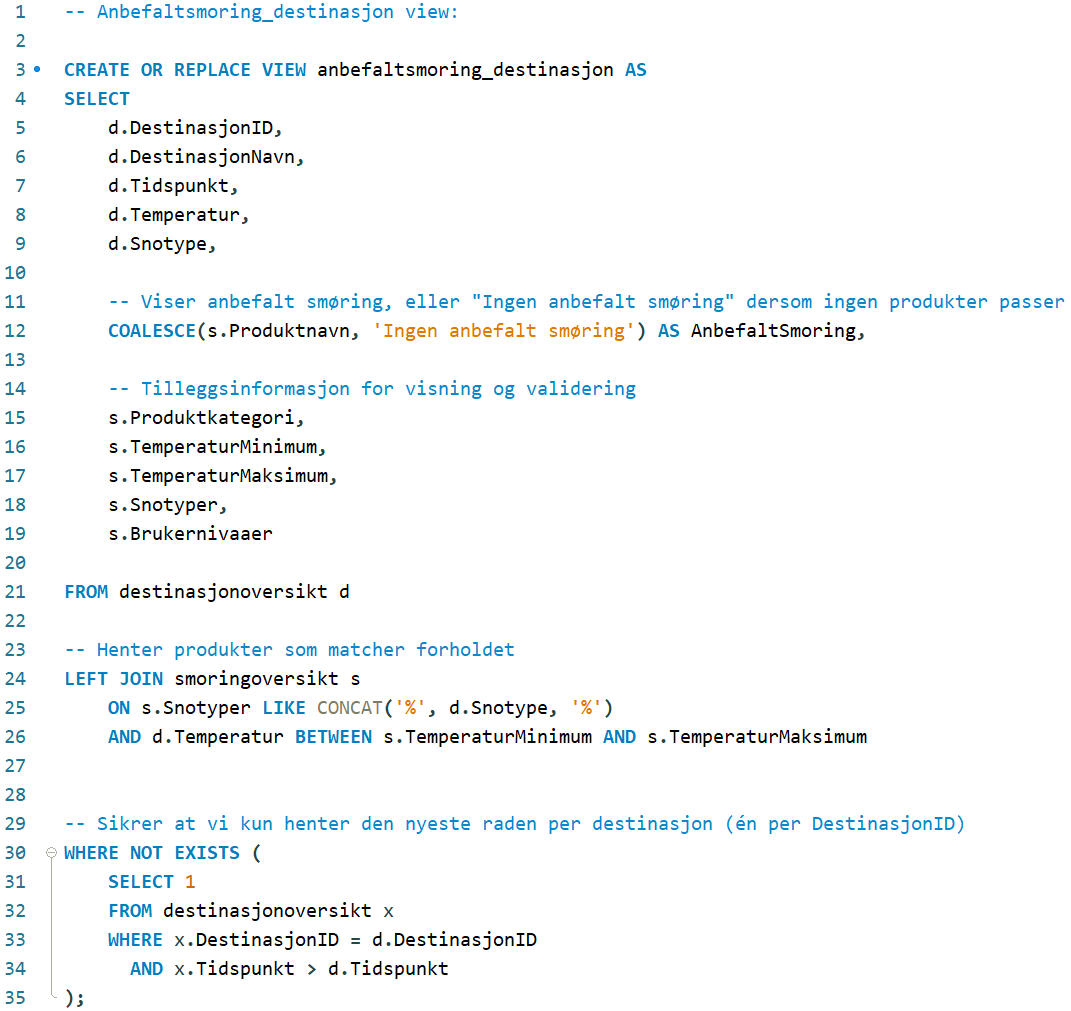
\includegraphics[width=\textwidth]{anbefaltsmoring_destinasjon.png}
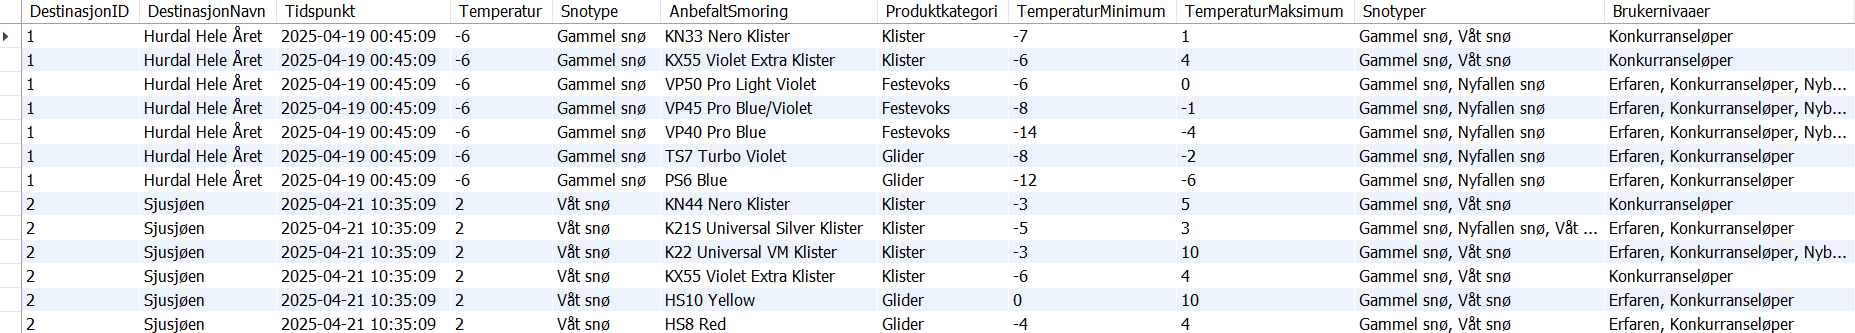
\includegraphics[width=\textwidth]{anbefaltsmoring_destinasjon_resultat.png}

Dette viewet sin hensikt er å hente ut den siste registrerte løypeforholdsmålingen per destinasjon, og viser hvilke smøringer som er anbefalt basert på registret snøtype og temperatur. Ved å bruke destinasjonoversikt får vi informasjonen vi trenger om snøtype og temperatur for hvert tidspunkt. Den kobles videre mot smoringoversikt for å finne alle produkter som støtter de gjeldende forholdene. Ved hjelp av LIKE og BETWEEN kobler vi alt opp mot temperatur og snøtype.

\subsection{Query: Anbefaltsmoring loypeforhold:}

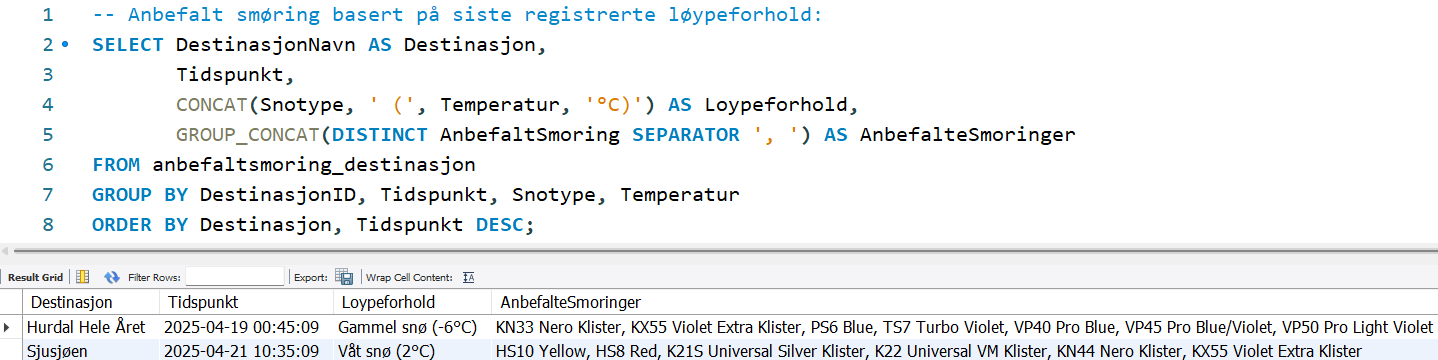
\includegraphics[width=\textwidth]{query_anbefaltsmoring_loypeforhold.png}

Spørringen sin hensikt er å vise hvilke smøringer som er anbefalt for en destinasjon basert på snøtype og temperatur. Denne spørringen bruker anbefaltsmoringdestinasjon viewet som kobler vær- og føreforhold mot anbefalte smøringer. Den kombinerer snøtype og temperatur for å vise når en smøring er aktuell. Deretter returnerer den alle anbefalinger per forhold og grupperer de tydelig. Den oppfyller følgende kravspesifikasjon fra oppgaven: "Systemet skal vise hvilke løypeforhold en smismøring er anbefalt for". 

\subsection{Query: Alternativsmoring originalsmoring:}

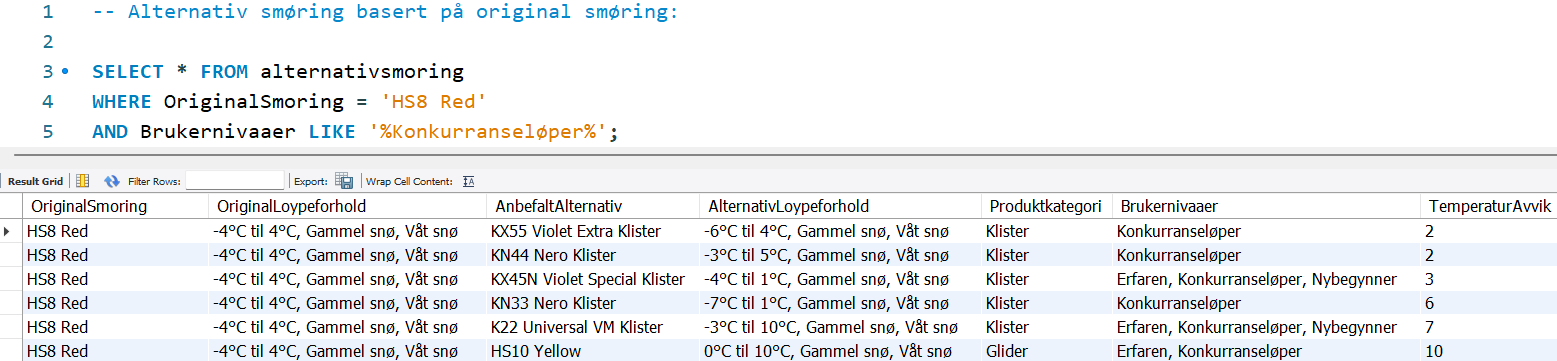
\includegraphics[width=\textwidth]{query_alternativsmoring.png}

Spørringen sin hensikt er å vise hvilke smøringer som er anbefalt for en destinasjon basert på snøtype og overlappende temperatur. Denne spørringen bruker alternativsmoring viewet som beregner avvik i temperaturintervall og filtrerer på snøtype. Den gir brukeren muligheten til å få anbefalt en alternativ smøring dersom den opprinnelige smøringen ikke er tilgjengelig. Resultatet returneres med sortering basert på temperaturavviket - jo lavere avvik, jo bedre alternativ. Den oppfyller følgende kravspesifikasjon fra oppgaven: "Systemet skal vise hvilke alternativer som finnes for spesifikke fohold".

\subsection{Query: Søkemekanisme:}

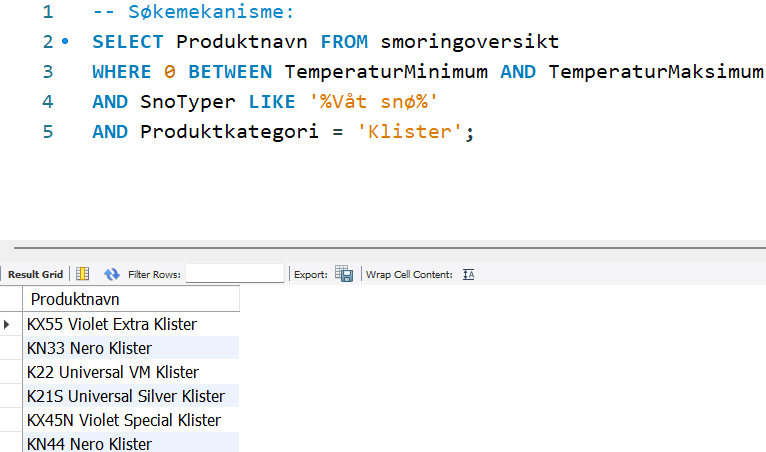
\includegraphics[width=\textwidth]{query_sokemekanisme.png}

Spørringen sin hensikt er å filtrere smøringer basert på spesifikke forhold: temperatur, snøtype og produktkategori. Denne spørringen matcher registrert temperatur mot produktets temperaturintervall. Videre krever den at snøtypen er støttet av produktet og at valgt kategori stemmer overens med produktet. Den oppfyller følgende kravspesifikasjon fra oppgaven: "Systemet skal tillate brukere å søke etter skismøringer basert på følgende kriterier: Temperaturintervall, snøtype, smørekategori. Systemet skal returnere en liste over alternative skismøringer som matcher søkekriteriene". 

\section{Kravspesifikasjon:}

\subsection{Funksjonelle krav:}

\begin{itemize}
	\item Skismøringregistrering: Håndteres gjennom INSERT INTO smoring(Produktnavn, Produktkategori, Produktnummer, Produktbeskrivelse) hvor produktegenskaper må knyttes mot smoringsid vha. INSERT INTO produktegenskaper(SmoringID, BrukernivaID, SnotypeID, TemperaturMinimum, TemperaturMaksimum). Unngår duplikater i smoring- og produktegenskaper-tabell vha. UNIQUE(), og validerer data som skal legges til i produktegenskaper vha. CHECK(). Testet ok.
	\item Løypeforhold: Hånteres på samme måte som over, men i loypeforhold-tabellen. Testet ok.
	\item Søkemekanisme: Håndteres gjennom query mot view: smoringoversikt. Testet ok.
	\item Oppdatering og sletting: Kan gjøres manuelt med INSERT INTO, men ser for oss at dette kan gjøres smidigere via frontend-løsning. Hva gjelder sletting har vi benyttet oss av ON DELETE CASCADE på relevante fremmednøkler, f.eks. fra produktegenskaper til smoring for å sikre at hvis en smøring fjernes, slettes også de tilkoblede egenskapene. Testet ok.
	\item Visning av informasjon:  Opprettet egnede views etter vårt syn. Testet ok.
\end{itemize}

\subsection{Ikke-funksjonelle krav:}

\begin{itemize}
	\item Brukervennlighet: Vi mener at strukturen i vår database nå er tilrettelagt på god måte med tanke på brukervennlighet, tenker da primært på views som en frontend-utvikler kan dra nytte av (ferdige spørringer hvor sluttbruker legger inn data de ønsker å søke på f.eks. dropdown på brukernivå e.l) 
	\item Tilgjengelighet/ytelse/skalerbarhet: Det vil være mulig å utvide databasen etter behov (f.eks. med en tabell for brukere, automatisk innhenting av temperatur mot destinasjon osv.) 
	\item Sikkerhet: Tilgangskontroll vha. GRANT X PRIVILEGES ON database TO enten enkeltbrukere eller brukergrupper, hvor X er hvilke tilganger som skal gis.
\end{itemize}

% section  (end)
\end{document}
